\chapter{Testování}\label{chapter:testovani}
% Nedílnou součástí vývoje softwaru je testování. Testování bylo rozděleno do dvou vrstev. Základní vrstvou jsou unit testy. Pro tvorbu těchto testů byl použit framework JUnit 5. Druhou vrstvou jsou integrační testy, které jsou implementovány pomoci funkcionality, kterou poskytuje framework Spring.
% Testování je nedílnou součástí implementace libovolného softwaru a je jeho velice důležitou částí. V rámci této bakalářské práce testům byla věnovaná řádná pozornost, proto bylo vyřešeno věnovat testům samostatnou kapitolu.
V této kapitole bude popsán proces testování a doplňující funkce zjednodušující proces testování. Také bude popsáno pokrytí kódů testy.

\section{Tagy}\label{testovani:tagy}
    Tagy už byly zmíněny v sekci \ref{navrh:testovani}, ale jejich chování nebylo podrobně popsáno. Nyní si tedy popíšeme chování tagů a proč je potřebujeme. 
    
    Tagy označují jednotlivé testy nebo celé testovací třídy pomocí obyčejného textového řetězce (viz obrázek \ref{code:tag-junit-5}). Obsah řetězce může být libovolný. Za účelem pohodlnějšího využití tagů byly zvoleny řetězce, které popisují konkrétní aspekt chování testu, například pomalý test nebo integrační test. Při spouštění testů pomocí frameworku JUnit můžeme definovat testy, které bychom potřebovali spustit pomocí těchto předem definovaných tagů.
    
    Stejného výsledku bychom mohli dosáhnout pomocí třídění testů do různých složek, ale podstatný rozdíl mezi těmito postupy je v tom, že jeden test může mít několik tagů najednou a přidání nebo odstranění tagu je jednoduché . Například test může být anotován jako pomalý integrační test a zároveň jako pomalý test proto, že provádí databázovou transakci. Dosáhnout stejného výsledku pomocí třídění testů do specifických složek je náročnější a nedovoluje umístit test do několika složek najednou.
    \begin{figure}
        \begin{minted}{java}
@Tags(
        Tag("integration_test")
)
        \end{minted}
        \caption{Příklad tagu frameworku JUnit 5} 
        \label{code:tag-junit-5}
    \end{figure}
    
    Tagy jsou jenom textové řetězce, je zde tedy velká pravděpodobnost překlepu při implementaci velkého počtu testů\footnote{V době odevzdání bakalářské práce bylo implementováno 126 testů v 25 třídách.}. Proto byly definovány vlastní anotace s předem definovanými tagy:
    \begin{itemize}
            \item \verb|IntegrationTest|, který má tag obsahující text \enquote{integration\_test};
            \item \verb|SecurityTest|, který má tag obsahující text \enquote{security\_test};
            \item \verb|SlowTest|, který má tag obsahující text \enquote{slow\_test};
            \item \verb|UnitTest|, který má tag obsahující text \enquote{unit\_test}.
    \end{itemize}
    
    \begin{figure}
        \begin{minted}{java}
/**
 * Specifies test as a Integration test.
 */
@Target(allowedTargets = [
        AnnotationTarget.FUNCTION,
        AnnotationTarget.ANNOTATION_CLASS,
        AnnotationTarget.CLASS
])
@Retention(AnnotationRetention.RUNTIME)
@MustBeDocumented
@Tags(
        Tag("integration_test")
)
annotation class IntegrationTest
        \end{minted}
        \caption{Příklad třídy \texttt{Annotation} zaměňující tag s textem \enquote{integration\_test}} 
        \label{code:annotation-class}
    \end{figure}
    Anotace mají stejnou implementaci a liší se pouze pomocí textu uvnitř tagů. Kotlin poskytuje podporu pro vytváření vlastních anotací, proto byla využita vestavěná třída \verb|anotation| (viz obrázek \ref{code:annotation-class}). Výsledné anotace jsou implementovány takovým způsobem, že pomocí nich je možné anotovat nejen testové metody, ale i celé třídy. Pak se anotace aplikuje na každý test, který obsahuje anotovaná třída. Také je možné anotovat i jiné anotace.

    \begin{figure}
        \begin{minted}{groovy}
tasks.test {
    useJUnitPlatform()
    testLogging {
        events 'PASSED', 'FAILED', 'SKIPPED'
    }

    maxHeapSize = "1G"
}

task unitTests(type: Test) {
    useJUnitPlatform {
        includeTags 'unit_test'
    }
    testLogging {
        events 'PASSED', 'FAILED', 'SKIPPED'
    }
}

task integrationTests(type: Test) {
    useJUnitPlatform {
        includeTags 'integration_test'
    }
    testLogging {
        events 'PASSED', 'FAILED', 'SKIPPED'
    }
}
        \end{minted}
        \caption{Úkoly pro spouštění testů} 
        \label{code:gradle-tests}
    \end{figure}
    Pro spouštění testů je potřeba využít nástroj pro automatizaci sestavování programu -- Gradle, který byl podrobně popsán v sekci \ref{resere:build} . Testy jsou rozděleny podle jejich typu pomocí tagů, proto byla přidána možnost, nejenom spustit všechny testy najednou, ale i spustit jenom unit testy nebo jenom integrační testy (viz obrázek \ref{code:gradle-tests}). Kombinací tagů je mnohem více, ale konfigurační soubor obsahuje jenom konfigurace, které potřeboval autor této práce během vývoje. 
    Přidat další konfigurace však není složité. Je potřeba pouze okopírovat předchozí konfiguraci v konfiguračním souboru a změnit seznam tagů podle potřeby. Seznam tagů je také možné doplnit. Všechny aktuální tagy se nacházejí ve složce \verb|src/test/kotlin/cz/cvut/fit/sp/rozvody/annotation/tag|~.
    
    Spuštění testů není omezené příkazovým řádkem. Testy je také možné spustit pomocí vývojového prostředí nebo jiných nástrojů. Můžeme použít například vývojové prostředí IntelliJ IDEA. 
    % Během vývoje velkých projektů zpouštění testů je významným problémem pro programátory. 
    % Framework JUnit 5 poskytuje možnost označovat metody a třídy pomocí tagu.
\section{Zobrazování testů}\label{testovani:zobrazovani}
    % TODO v pripade ze pobezi testy pres IDEA. Pres terminal nefunguje CamelCaseGenerator
    Správné a pochopitelné zobrazování názvů testů zjednodušuje proces testování. Proto před začátkem implementaci testů bylo navrhnuto pravidlo pro zobrazování testů. Název testu má obsahovat v stručný popis toho, co by měl otestovat. 
    
    \begin{figure}\centering
	   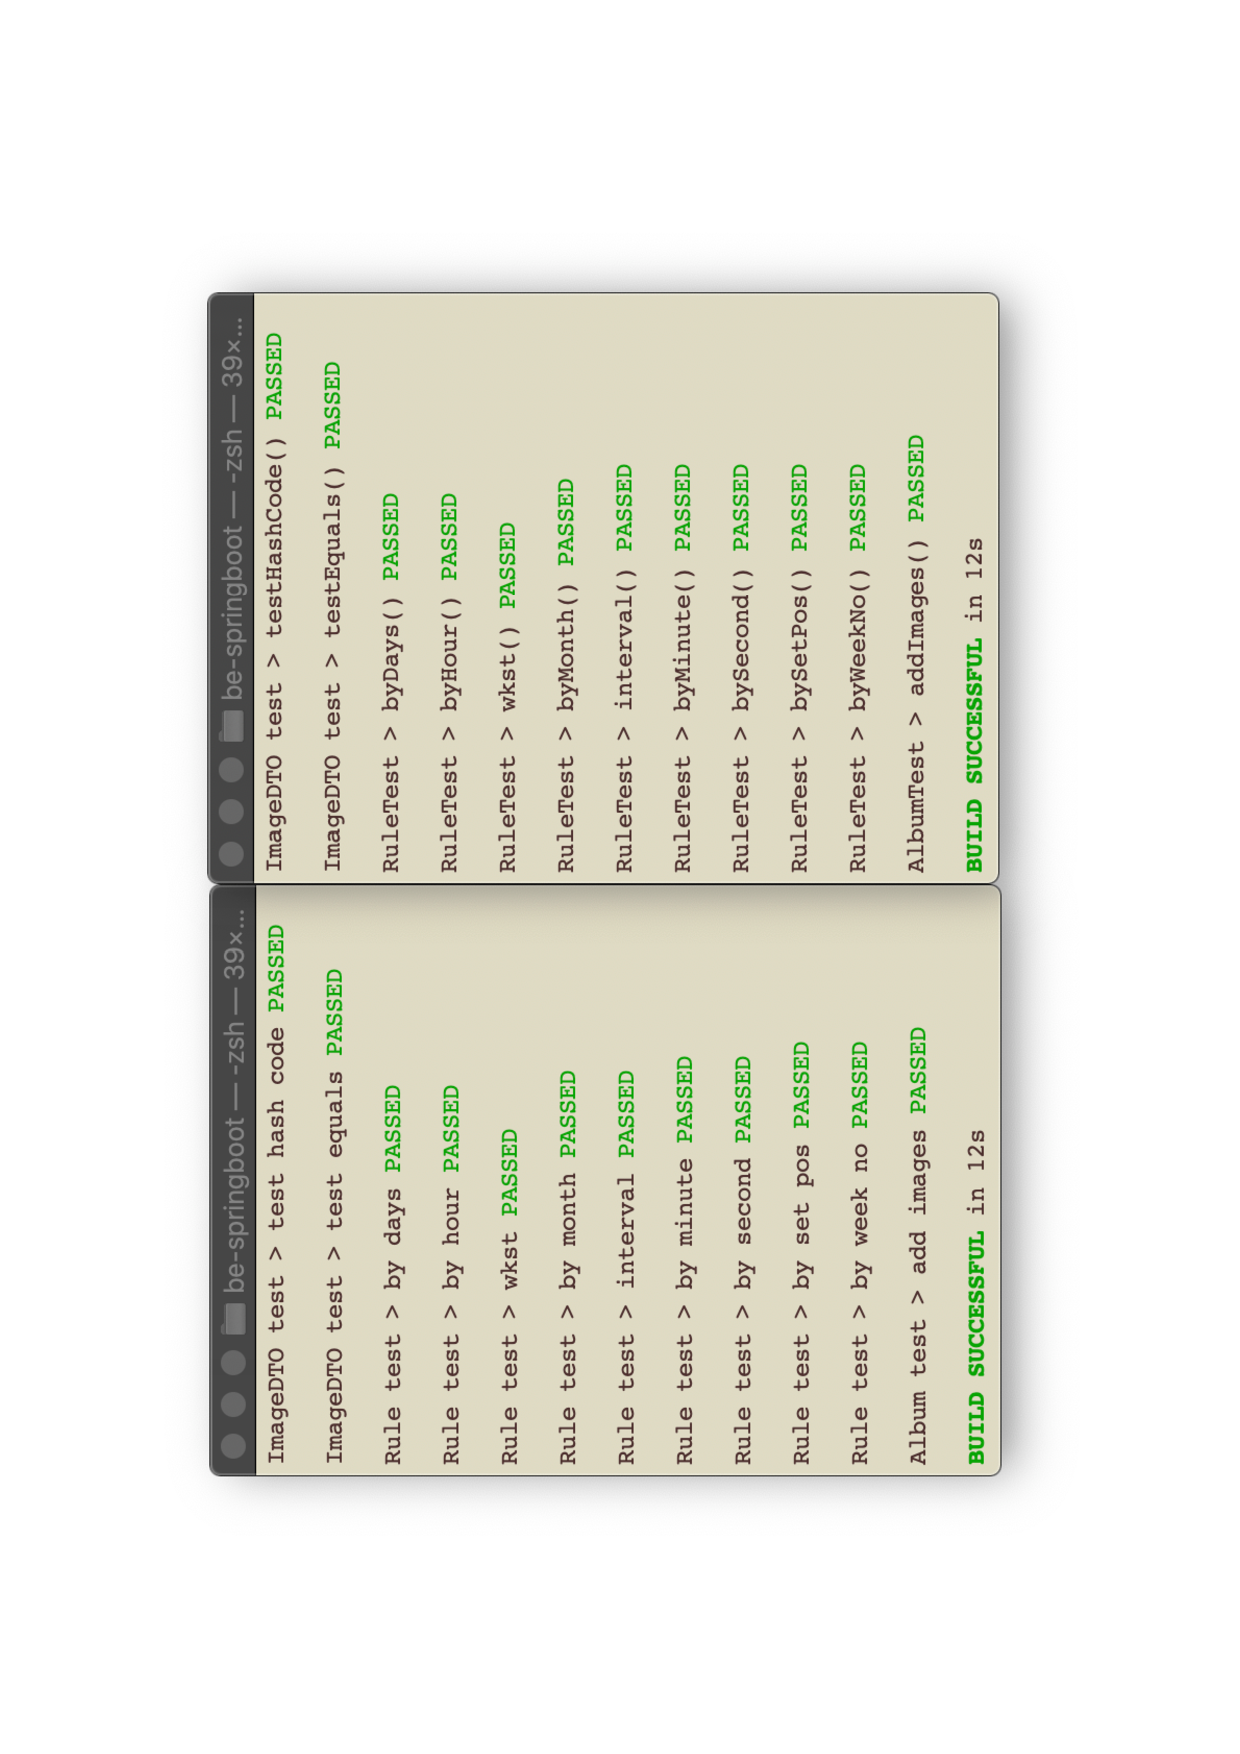
\includegraphics[angle=-90, width=1.0\textwidth]{pdfs/pretty-tests-comparison}
	   \caption[Srovnaní zobrazováni kódu]{Příklad vypisování testů pomocí generátoru (4.4a) a bez využití generátoru (4.4b)}\label{image:pretty-tests-comparison}
    \end{figure}
    Pro čitelnější zobrazování byl implementován generátor transformující jméno testu nebo jméno třídy do čitelnější podoby (viz obrázek \ref{image:pretty-tests-comparison}). Princip fungování je založen na překladu názvu z \textit{camel case} na obyčejný text s mezerami. Výsledné názvy testů nebo tříd neobsahují žádné zbytečné symboly\footnote{Za zbytečné symboly jsou považovány prázdné závorky na konci názvu metody atd.}. Pro pohodlné využití generátoru byla implementována anotace, která je aplikovatelná na třídy a metody. Anotace aktivuje generátor pro všechny testy, které třída obsahuje nebo pro konkrétní test, na který byla aplikována.
    
    V případě, že název metody obsahuje text, který by se neměl korektně transformovat, potřebujeme použít anotaci \verb|DisplayName| a v závorkách této anotace uvést text, který by měl být zobrazen. Tento název přepisuje výsledek generátoru, proto může být tato anotace použita ve třídě, která má anotaci generátoru. Příkladem takového nevhodného názvu může být třída se jménem \verb|ImageDTO|, která bude přeložena na \enquote{Image~d~t~o}, což není požadováným výsledkem.
    
\section{Unit testy}\label{testovani:unit}
    % Unit testy jsou zaměřené na otestování samostatně testovatelných metod a tříd
    Unit testy jsou zaměřené na otestování samostatně testovatelných metod a tříd. Všechny unit testy jsou anotovány jako unit testy (viz sekci \ref{testovani:tagy}) za účelem přidání možnosti spustit tyto testy zvlášť od ostatních testů. Žádný z testů není závislý na celém kontextu aplikace nebo její části, proto jsou všechny unit testy rychlé.
    
\section{Integrační testy}\label{testovani:intergacni}
    % TODO Integrační testy zaměřené na ověření správné komunikace mezi komponentami aplikace.
    Velká pozornost byla věnovaná integračním testům. Tyto testy ověřují, jestli jednotlivé komponenty aplikace pracují podle jejich návrhu. Testy jsou anotovány jako integrační testy (viz sekci \ref{testovani:tagy}) za účelem přidání možnosti spustit tyto testy zvlášť od ostatních, stejně jako unit testy. 
    
    Integrační testy vyžadují nahrání celého kontextu aplikace nebo jeho částí, proto jsou pomalejší než unit testy. Některé testy navíc mění kontext aplikace a vyžadují zrušení kontextu po dokončení jejich běhu. Takové testy jsou anotovány jako pomalé testy\footnote{Anotace \texttt{SlowTest}, obsahující tag \enquote{slow\_test}.}.
    
        \begin{figure}
        \begin{minted}{java}
mvc.perform(
        MockMvcRequestBuilders
            .post("/api/v1/comment")
            .contentType(MediaType.APPLICATION_JSON)
            .content(commentDTO.toString())
)
    .andExpect(status().isCreated)
    .andExpect(content().contentType(MediaType.APPLICATION_JSON))
    .andExpect(jsonPath("$.createdById", is(
        commentDTO.createdById.toInt()
        )))
    .andExpect(jsonPath("$.text", is(commentDTO.text)))
    .andExpect(jsonPath("$.createdAt", is(
        commentDTO.createdAt.format(
            DateTimeFormatter.ISO_LOCAL_DATE_TIME
            )
        )))

        \end{minted}
        \caption{Příklad použití nástroje MockMvc} 
        \label{code:mockmvc}
    \end{figure}
    Většina integračních testů je zaměřena na ověření správného fungování vrstvy řadičů (\textit{controller}). Testování se provádí pomocí nástroje MockMvc\cite{mock-mvc}, který poskytuje framework Spring. Nástroj umožňuje otestovat funkcionalitu aplikace bez jejího úplného nastartování. Příklad využití nastroje je na obrázku \ref{code:mockmvc}. Tento kód má za úkol otestovat, zda řadič správně vytváří instanci entity \textit{Comment}. Kontrola správnosti atributu se provádí na základě DTO, který se vrátí jako návratová hodnota.
    
    V rámci integračních testu byla také ověřena přístupová práva (viz sekci \ref{navrh:bezpecnost}). Při testování řadičů bylo zapnuto filtrování podle role přihlášeného uživatele. Každému testu patří jeden uživatel, který je nastaven pomocí uživatelského jména\footnote{Uživatelským jménem v systému je adresa elektronické pošty.}. V případě, že uživatel nemá dostatečná přístupová práva, řadič musí vrátit HTTP status s číslem 400\footnote{Bad Request.}.
    
\section{Samostatný profil pro testování}

    Testovaní aplikace vyžaduje vlastní nastavení, proto byl vytvořen samostatný profil, který odděluje testovací nastavení od nastavení produkce a vývoje. Profil má vlastní konfigurační soubor (\verb|application-test.properties|), obsahující nastavení databáze.
    
    Pro testování byla  využita stejná databáze jako i pro proces vývoje, za účelem kompletního a rychlého testování serveru. Databáze umožňuje rychle zrušit a vytvořit tabulky, což nám umožňuje rychle zrušit kontext aplikace mezi integračními testy.
    
    Profil pro testování má též vlastní implementaci pro \verb|UserDetailsService|\footnote{Základní rozhraní, které framework Spring využívá pro načítaní informací o uživateli.}, obsahující tři implicitní uživatele:
    \begin{itemize}
            \item \verb|root|, vlastnící role \enquote{ROLE\_USER} a \enquote{ROLE\_ROOT} 
            \item \verb|userEmail|, vlastnící role \enquote{ROLE\_USER}
            \item \verb|user2Email|, vlastnící role \enquote{ROLE\_USER}
    \end{itemize}
    Tyto implicitní uživatel jsou využity v integračních testech pro spouštění požadavků (\verb|request|) přes instanci MocMvc. Podrobněji byly integrační testy popsány v sekci \ref{testovani:intergacni}.
    
\section{Pokrytí kódu testy}\label{testovani:pokryti}
    % TODO V této sekci je uveden popis provedéní analýzy pokrýtí kódu testy.
    V této sekci bude popsáno pokrytí kódů testy a uvedeny statistiky. Za účelem zvýšení přesnosti provedené analýzy byly využity speciální nástroje pro zhodnocení pokrytí kódů.
    
    \subsection{JaCoCo}
    Prvním nástrojem, který byl využit pro analýzu testů, je JaCoCo. Tento nástroj byl podrobně popsán v sekci \ref{resere:testovani:jacoco} . V této sekci je uveden pouze proces analýzy a její výsledky.
    
    JaCoCo vyžaduje implementování vlastního úkolu\footnote{Konfigurovatelný úkol pro nástroj Gradle, například \texttt{test} nebo \texttt{build}.}(\verb|task|) v Gradle. Tento úkol byl nazván \verb|jacocoTestReport| a je možné jej spustit přes příkazový řádek. Generování výsledků závisí na spouštění klasického úkolu \verb|test| od Gradle. 
    
    Generování výsledků pokrytí testů bylo využito jako nápověda pro identifikování důležitého kódu nepokrytého testy. Proto byl úkol \verb|jacocoTestReport| spuštěn několikrát. Podle poslední verze výsledků, která byla spuštěna pro poslední verzi aplikace, 85 \% instrukcí je pokryté testy. Podrobné informace se můžete dozvědět v příloze \ref{dodatek:code-coverage}.
    % vestaveny junit engine v IntelifIDEA prestal fingovat po dosazeni velkeho poctu testu
    \subsection{IntelliJ IDEA}
    Druhým testovacím nástrojem, který byl využit pro zjištění pokrytí kódů testy, je InteliJ~IDEA. Podrobněji byl tento nástroj popsán v sekci \ref{resere:testovani:intellij-idea} . 
    
    Tento nástroj byl také využit jako pomocný nástroj při implementaci testů. V této sekci budou uvedeny jenom výsledky posledního spuštění pro poslední verzi aplikace. Kompletní informace o výsledcích jsou k nalezení v příloze \ref{dodatek:code-coverage}.
    
    IntelliJ IDEA poskytuje nepatrně odlišnou informaci o pokrytí kódů než nástroj JaCoCo. Podle výsledků jsou pokryté testy:
    \begin{itemize}
            \item 72,6 \% tříd
            \item 90,1 \% metod
            \item 89,3 \% řádek kódů
    \end{itemize}